\documentclass[submit]{harvardml}

% FDV: Update front matter -- years, dates, references to book sections, etc.
\course{CS181-S22}
\assignment{Assignment \#5}
\duedate{11:59pm EST, April 8, 2021}

\newcommand{\attr}[1]{\textsf{#1}}
\usepackage[OT1]{fontenc}
\usepackage[colorlinks,citecolor=blue,urlcolor=blue]{hyperref}
\usepackage[pdftex]{graphicx}
\usepackage{subfig}
\usepackage{framed}
\usepackage{fullpage}
\usepackage{amsmath}
\usepackage{amssymb}
\usepackage{color}
\usepackage{todonotes}
\usepackage{listings}
\usepackage{common}
\usepackage{bm}
\usepackage{enumitem}
\usepackage{tikz}
\usetikzlibrary{positioning,shapes,arrows}
\usepackage{xifthen}
\usepackage{pythonhighlight}
\usepackage{soul}

\usepackage[mmddyyyy,hhmmss]{datetime}

\definecolor{verbgray}{gray}{0.9}

\lstnewenvironment{csv}{
  \lstset{backgroundcolor=\color{verbgray},
  frame=single,
  framerule=0pt,
  basicstyle=\ttfamily,
  columns=fullflexible}}{}

\newcommand{\TODO}{{\color{red}TODO }}

\begin{document}


\begin{center}
{\Large Homework 5: EM with Mixtures, PCA, and Graphical Models}\\
\end{center}

This homework assignment will have you work with EM for mixtures, PCA,
and graphical models. We encourage you to read sections 9.4 and 8.2.5 of the course textbook.

Please type your solutions after the corresponding problems using this
\LaTeX\ template, and start each problem on a new page.

Please submit the \textbf{writeup PDF to the Gradescope assignment `HW5'}. Remember to assign pages for each question.

Please submit your \textbf{\LaTeX\ file and code files to the Gradescope assignment `HW5 - Supplemental'}. 


\newpage
\begin{problem}[Expectation-Maximization for Gamma Mixture Models, 25pts]

In this problem we will explore expectation-maximization for a Categorical-Gamma Mixture model.

Let us suppose the following generative story for an observation $x$: first one of $K$ classes is randomly selected, and then the features $x$ are sampled according to this class. If $$z \sim \operatorname{Categorical}(\btheta)$$ indicates the selected class, then $x$ is sampled according to the class or ``component'' distribution corresponding to $z$. (Here, $\btheta$ is the mixing proportion over the $K$ components: $\sum_k \theta_k = 1$ and $ \theta_k > 0$). In this problem, we assume these component distributions are gamma distributions with shared shape parameter but different rate parameters: $$x | z \sim \operatorname{Gamma}(\alpha, \beta_k).$$

In an unsupervised setting, we are only given a set of observables as our training dataset: $\mathcal D = \{x_n\}_{n=1}^N$. The EM algorithm allows us to learn the underlying generative process (the parameters $\btheta$ and $\{\beta_k\}$) despite not having the latent variables $\{z_n\}$ corresponding to our training data.

\vspace{2em}

\begin{enumerate}

  \item \textbf{Intractability of the Data Likelihood} We are
    generally interested in finding a set of parameters $\beta_k$ that
    maximizes the likelihood of the observed data: $$\log
    p(\{x_n\}^N_{n=1}; \btheta, \{\beta_k\}^K_{k = 1}).$$ Expand the data
    likelihood to include the necessary sums over observations
    $x_n$ and to marginalize out the latents
    $\boldz_n$. Why is optimizing this likelihood directly
    intractable?

\item \textbf{Complete Data Log Likelihood} The complete dataset
  $\mathcal D = \{(x_n, \boldz_n)\}_{n=1}^N$ includes latents $\boldz_n$. Write
  out the negative complete data log likelihood: $$\mcL(\btheta, \{\beta_k\}^K_{k=1}) =  -\log p(\mathcal D; \btheta, \{\beta_k\}^K_{k=1}).$$

  Apply the power trick and simplify your expression using indicator elements $z_{n
  k}$.\footnote{The ``power trick'' is used when terms in a PDF are raised to the power of indicator components of a one-hot vector.  For example, it allows us to rewrite $p(\boldz_n ;  \btheta) = \prod_k \theta_k^{z_{nk}}$.} Notice that optimizing this loss is now computationally tractable if we know $\boldz_n$.

  (Continued on next page.)

\end{enumerate}

\end{problem}

\newpage


\begin{framed}
\noindent\textbf{Problem 1} (cont.)\\
\begin{enumerate}
\item[3.] \textbf{Expectation Step} Our next step is to introduce a
  mathematical expression for $\boldq_n$, the posterior over the
  hidden component variables~$\boldz_n$ conditioned on the observed data
  $x_n$ with fixed parameters.
That is:
  \begin{align*}
    \textbf{q}_n &= \begin{bmatrix}
      p(\boldz_n =\boldC_1| x_n; \btheta, \{ \beta_k \}^K_{k=1}) \\
      \vdots \\
      p(\boldz_n =\boldC_K| x_n; \btheta, \{ \beta_k \}^K_{k=1})
    \end{bmatrix}.
  \end{align*}
  %
%
  Write down and simplify the expression for
  $\boldq_n$.  Note that because the $\boldq_n$ represents the
  posterior over the hidden categorical variables $\boldz_n$, the
  components of vector $\boldq_n$ must sum to 1.
  The main work is to find an expression for $p(\boldz_n|x_n; \btheta, \{\beta_k\}^K_{k=1})$  for any choice of $\boldz_n$; i.e., for any 1-hot encoded $\boldz_n$. With this, you can then construct the different components that make up the vector $\boldq_n$.
  
\item[4.] \textbf{Maximization Step}
Using the~$\boldq_n$ estimates from the Expectation Step, derive an update for maximizing the expected complete data log likelihood in terms of $\btheta$ and $\{ \beta_k \}^K_{k=1}$.

\begin{enumerate}
    \item Derive an expression for the expected complete data log likelihood using $\boldq_n$.
    \item Find an expression for $\btheta$ that maximizes this expected complete data log likelihood. You may find it helpful to use Lagrange multipliers in order to enforce the constraint $\sum \theta_k = 1$. Why does this optimal $\btheta$ make intuitive sense?
    \item Find an expression for $\beta_k$ that maximizes the expected complete data log likelihood.  Why does this optimal $\beta_k$  make intuitive sense?
\end{enumerate}
    
\item[5.] Suppose that this had been a classification problem. That is,
  you were provided the ``true'' components $\boldz_n$ for each
  observation $x_n$,
  and you were going to perform the classification by
  inverting the provided generative model (i.e. now you're predicting $\boldz_n$ given $x_n$). Could you reuse any of
  your derivations above to estimate the parameters of the model?
  

\item[6.] Finally, implement your solution in \texttt{p1.ipynb} and attach the final plot below.

{\bfseries You will recieve no points for code not included below.}
\end{enumerate}
  
\end{framed}

\newpage
\subsection*{Solution}

\begin{enumerate}
  \item The likelihood expands to
	\begin{align*}
	 	\log p(\{x_n\}^N_{n=1}; \btheta, \{\beta_k\}^K_{k = 1})
	 	&= \log \prod_{n=1}^N p(x_n; \btheta, \{\beta_k\}^K_{k = 1}) \\
	 	&= \log \prod_{n=1}^N \sum_{k=1}^K p(x_n, z_{nk}; \btheta, \{\beta_k\}^K_{k = 1}) \\
	 	&= \sum_{n=1}^N \log \left[\sum_{k=1}^K p(x_n, z_{nk}; \btheta, \{\beta_k\}^K_{k = 1})\right].
	\end{align*}
	Optimizing this likelihood directly is intractable because of the summation over the $K$ classes inside of the logarithm, which precludes an analytical solution.
  
  \item The negative complete data log likelihood expands to
	\begin{align*}
		\mcL(\btheta, \{\beta_k\}^K_{k=1})
		&=  -\log p(\mathcal D; \btheta, \{\beta_k\}^K_{k=1}) \\
		&=  -\sum_{n=1}^N \log p(x_n, \boldz_n; \btheta, \{\beta_k\}^K_{k=1}) \\
		&= -\sum_{n=1}^N \log [p(x_n | \boldz_n; \{\beta_k\}^K_{k=1})p(\boldz_n; \btheta)] \\
		&= -\sum_{n=1}^N \log p(x_n | \boldz_n; \{\beta_k\}^K_{k=1}) + \log p(\boldz_n; \btheta).
	\end{align*}
	Applying the power trick,
		\begin{align*}
		\mcL(\btheta, \{\beta_k\}^K_{k=1})
		&= -\sum_{n=1}^N \left[ \log \prod_{k=1}^K p(x_n|\boldz_n = \boldC_k; \{\beta_k\}^K_{k=1})^{z_{nk}} + \log \prod_{k=1}^K \theta_k^{z_{nk}} \right] \\
		&= -\sum_{n=1}^N \sum_{k=1}^K z_{nk} \log p(x_n|\boldz_n = \boldC_k; \{\beta_k\}^K_{k=1}) + z_{nk} \log \theta_k.
	\end{align*}
  
  \item Using Bayes' Rule and the power trick,
  \begin{align*}
  	p(\boldz_n|x_n; \btheta, \{\beta_k\}^K_{k=1})
  	&=\frac{\prod_{k=1}^K \left(p(x_n|\boldz_n=\boldC_k; \{\beta_k\}^K_{k=1})\theta_k\right)^{z_{nk}}}{\sum_{k=1}^Kp(x_n|\boldz_n=\boldC_k; \{\beta_k\}^K_{k=1})\theta_k} \\
  	 &=\frac{\prod_{k=1}^K (p(x_n|\boldz_n=\boldC_k; \{\beta_k\}^K_{k=1}))^{z_{nk}} \prod_{k=1}^K (\theta_k)^{z_{nk}}}{\sum_{k=1}^Kp(x_n|\boldz_n=\boldC_k; \{\beta_k\}^K_{k=1})\theta_k}.
  \end{align*}
	The soft assignment value for a particular class $k$ is
	\begin{align*}
		q_{nk} &= p(\boldz_n = \boldC_k |x_n; \btheta, \{\beta_k\}^K_{k=1}) \\
		&= \frac{p(x_n|\boldz_n = \boldC_k; \{\beta_k\}^K_{k=1})p(\boldz_n = \boldC_k; \btheta)}{\sum_{k=1}^Kp(x_n|\boldz_n = \boldC_k; \{\beta_k\}^K_{k=1})p(\boldz_n = \boldC_k; \btheta)} \\
		&= \frac{p(x_n|\boldz_n = \boldC_k; \{\beta_k\}^K_{k=1})\theta_k}{\sum_{k=1}^Kp(x_n|\boldz_n = \boldC_k; \{\beta_k\}^K_{k=1})\theta_k}.
	\end{align*}
	Therefore,
	 \begin{align*}
		\textbf{q}_n &= \begin{bmatrix}
			\frac{p(x_n|\boldz_n = \boldC_1; \{\beta_k\}^K_{k=1})\theta_1}{\sum_{k=1}^Kp(x_n|\boldz_n = \boldC_k; \{\beta_k\}^K_{k=1})\theta_k} \\
			\vdots \\
			\frac{p(x_n|\boldz_n = \boldC_K; \{\beta_k\}^K_{k=1})\theta_K}{\sum_{k=1}^Kp(x_n|\boldz_n = \boldC_k; \{\beta_k\}^K_{k=1})\theta_k}
		\end{bmatrix}.
	\end{align*}
  
  \item 
    \begin{enumerate}
      \item The expected complete data log likelihood is
      \begin{align*}
      &\mathbb{E}_{\{\boldz_n\}_{n=1}^N | \{x_n\}_{n=1}^N} \left[\log p(\mathcal D; \btheta, \{\beta_k\}^K_{k=1})\right] \\
      &= \mathbb{E}_{\{\boldz_n\}_{n=1}^N | \{x_n\}_{n=1}^N} \left[\sum_{n=1}^N \log p(x_n|\boldz_n; \{\beta_k\}^K_{k=1}) + \log p(\boldz_n; \btheta)\right] \\
	  &= \sum_{n=1}^N \mathbb{E}_{\boldz_n | x_n} \left[\log p(x_n|\boldz_n; \{\beta_k\}^K_{k=1}) + \log p(\boldz_n; \btheta)\right] \\
	  &= \sum_{n=1}^N \sum_{k=1}^K p(\boldz_n = \boldC_k|x_n; \btheta, \{\beta_k\}^K_{k=1}) (\log p(x_n|\boldz_n = \boldC_k; \{\beta_k\}^K_{k=1}) + \log p(\boldz_n = \boldC_k; \btheta)) \\
	  &= \sum_{n=1}^N \sum_{k=1}^K q_{nk} \log p(x_n|\boldz_n = \boldC_k; \{\beta_k\}^K_{k=1}) + q_{nk} \log \theta_k,
      \end{align*}
      where $q_{nk}$ is the probability computed in the E-step.

      \item Use Lagrange multipliers on the expected complete data log likelihood from the previous part with the constraint $\sum_k \theta_k - 1 = 0$. The Lagrangian is
      $$\sum_{n=1}^N \sum_{k=1}^K \left(q_{nk} \log p(x_n|\boldz_n = \boldC_k; \{\beta_k\}^K_{k=1}) + q_{nk} \log \theta_k\right) - \lambda\left(\sum_{k=1}^K \theta_k - 1\right).$$
      Optimizing by differentiating with respect to $\theta_k$ and setting equal to zero, noting that we treat the $q_{nk}$ as fixed in the M-step:
	  \begin{align*}
		\sum_{n=1}^N \frac{q_{nk}}{\theta_k} - \lambda = 0 \\
	  	\theta_k = \frac{\sum_{n=1}^N q_{nk}}{\lambda}.
	  \end{align*}
  	  Summing over $k$, recalling that $\sum_k \theta_k = 1$,
  	  	$$\sum_{k=1}^K \theta_k = \frac{\sum_{k=1}^K \sum_{n=1}^N q_{nk}}{\lambda} = 1 \Rightarrow \lambda = \sum_{k=1}^K \sum_{n=1}^N q_{nk} = \sum_{n=1}^N \sum_{k=1}^K q_{nk}.$$
 	Substituting this expression for $\lambda$ back into our expression for $\theta_k$,
 	$$\theta_k = \frac{\sum_{n=1}^N q_{nk}}{\sum_{n=1}^N \sum_{k=1}^K q_{nk}} = \frac{\sum_{n=1}^N q_{nk}}{N}.$$
 	Therefore the optimal $\btheta$ is
 	$$\left(\frac{\sum_{n=1}^N q_{n1}}{N}, \ldots, \frac{\sum_{n=1}^N q_{nK}}{N}\right).$$
 	This makes intuitive sense because the optimal $\theta_k$ for each class is proportional to the sum of all of the data points' soft assignment probabilities for that class.
 	
      \item 
      
      % old math using betas as scale rather than rate
      \begin{comment}
      Substituting the gamma PDF into the expected complete data log likelihood gives
      $$\sum_{n=1}^N \sum_{k=1}^K q_{nk} \log \frac{(x_n)^{\alpha-1}e^{-x_n/\beta_k}}{(\beta_k)^\alpha\Gamma(\alpha)} + q_{nk} \log \theta_k$$
      $$\sum_{n=1}^N \sum_{k=1}^K q_{nk} \left((\alpha - 1)\log x_n - \frac{x_n}{\beta_k} - \alpha \log \beta_k - \log \Gamma(\alpha)\right)+ q_{nk} \log \theta_k$$
      Optimizing by differentiating with respect to $\beta_k$ and setting equal to zero, we have
      $$\sum_{n=1}^N q_{nk} \frac{x_n}{\beta_k^2} - q_{nk} \frac{\alpha}{\beta_k} = 0$$	$$\beta_k = \frac{1}{\alpha} \cdot \frac{\sum_{n=1}^N q_{nk} x_n}{\sum_{n=1}^N q_{nk}}.$$
      This optimal $\beta_k$ makes intuitive sense because it is $1/\alpha$ times the weighted average of all of the $x_n$, where each $x_n$ is weighted by how likely it currently is to belong to class $k$.
      \end{comment}
  
      Substituting the gamma PDF into the expected complete data log likelihood gives
	  $$\sum_{n=1}^N \sum_{k=1}^K q_{nk} \log \frac{(x_n)^{\alpha-1}e^{-\beta_k x_n}(\beta_k)^\alpha}{\Gamma(\alpha)} + q_{nk} \log \theta_k$$
	  $$\sum_{n=1}^N \sum_{k=1}^K q_{nk} \left((\alpha - 1)\log x_n - \beta_kx_n + \alpha \log \beta_k - \log \Gamma(\alpha)\right)+ q_{nk} \log \theta_k$$
	  Optimizing by differentiating with respect to $\beta_k$ and setting equal to zero, we have
	  $$\sum_{n=1}^N -q_{nk} x_n + q_{nk} \frac{\alpha}{\beta_k} = 0$$
	  $$\beta_k = \alpha \cdot \frac{\sum_{n=1}^N q_{nk}}{\sum_{n=1}^N q_{nk} x_n}.$$
	  This optimal $\beta_k$ makes intuitive sense because it is $\alpha$ times the reciprocal of the weighted average of all of the $x_n$, where each $x_n$ is weighted by how likely it currently is to belong to class $k$.

    \end{enumerate}
  \item 
  Yes, we could reuse the derivated parameter estimates by substituting $\boldq_n$ with $\boldz_n$ for each data point, making $q_{nk}=1$ for the true class $k$ and $q_{nk}=0$ for all other classes. This corresponds to predicting the true class with probability 1. This substitution gives the following MLE parameters:
  $$\theta_k = \frac{\sum_{n=1}^N q_{nk}}{N} =  \frac{\sum_{n=1}^N z_{nk}}{N},$$
  which is the empirical proportion of data points in class $k$, and
  $$\beta_k = \alpha \cdot \frac{\sum_{n=1}^N q_{nk}}{\sum_{n=1}^N q_{nk} x_n} = \alpha \cdot \frac{\sum_{n=1}^N z_{nk}}{\sum_{n=1}^N z_{nk} x_n}.$$
  which is $\alpha$ times the reciprocal of the empirical mean of data points in class $k$. These parameters can be used to approximate the joint distribution $p(x_n, \boldz_n; \btheta, \{\beta_k\}^K_{k = 1})$, which can in turn be used to predict $\boldz_n$ given $x_n$ using Bayes' rule, as we did in classification:
  $$p(\boldz_n = \boldC_k | x_n; \btheta, \{\beta_k\}^K_{k = 1}) = \frac{p(x_n, \boldz_n; \btheta, \{\beta_k\}^K_{k = 1})}{p(x_n; \btheta, \{\beta_k\}^K_{k = 1})} \propto p(x_n | \boldz_n = \boldC_k; \{\beta_k\}^K_{k = 1})p(\boldz_n = \boldC_k; \btheta).$$
  
  \item 
    Plot:

    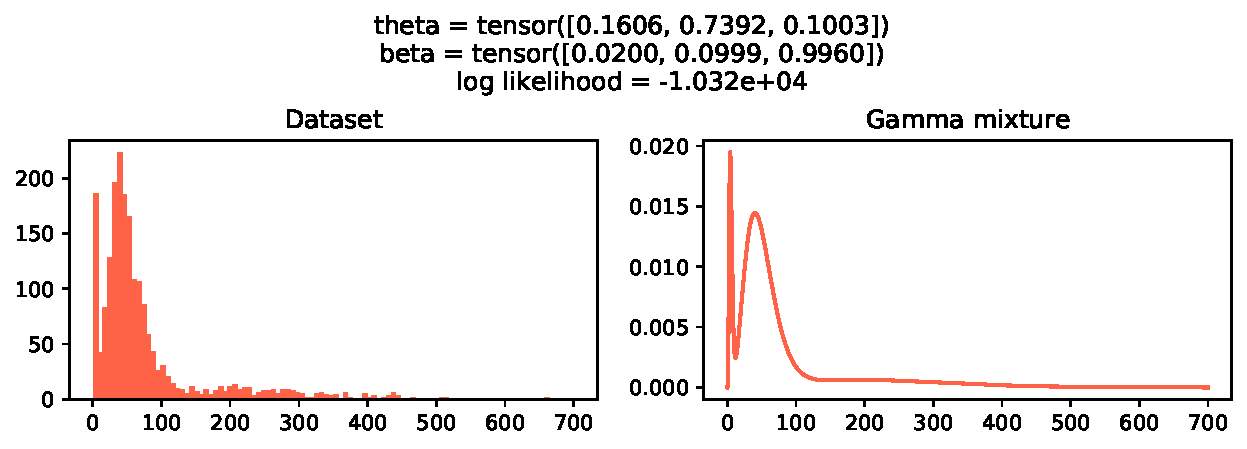
\includegraphics[width=\linewidth]{p1}

    Code:

    \begin{python}
def e_step(theta, betas):
    log_q = ds.gamma.Gamma(alpha, betas).log_prob(x) + torch.log(theta)
    q = torch.exp(log_q - log_q.logsumexp(dim=1, keepdim=True))
    return q


def m_step(q):
    q_sums = torch.sum(q, 0)
    theta_hat = q_sums / q.shape[0]
    beta_hats = alpha * q_sums / torch.sum(q * x, 0)
    return theta_hat, beta_hats


def log_px(x, theta, betas):
    non_log_ps = (ds.gamma.Gamma(alpha, betas).log_prob(x) + torch.log(theta)).exp()
    p = torch.log(non_log_ps.sum(1))
    return p


def run_em(theta, betas, iterations=1000):
    for _ in range(iterations):
        q = e_step(theta, betas)
        theta, betas = m_step(q)
    return theta, betas
    \end{python}
\end{enumerate}


\newpage

\begin{problem}[PCA, 15 pts]

% FDV: Here are the notes from last year.  I've already edited to make clear we want L2.  As noted below, we should also provide the baseline/reference to the pset 4 solutions in case they computed that wrong somehow.  
% 
% # problem 2 clarifications
% *NB: There was a lot of confusion about this problem, and we ended up accepting any form of comparison to PCA. Next year should clarify which norm students should use more explicitly (and maybe provide a baseline for students if the computation of the reconstruction error is different from what students calculated on pset4.)*
% 
% For Problem 2.3 (computing PCA reconstruction error), we will accept both the L1 and L2 norm and both summing over the errors for individual images and taking the mean of the errors (as long as you compute the error for K-Means the same way as you compute it for PCA). Apologies for the ambiguity in this question! 

  
For this problem you will implement PCA from scratch on the first 6000 images of the MNIST dataset. Your job is to apply PCA on MNIST and discuss what kind of structure is found. Implement your solution in \texttt{p2.ipynb} and attach the final plots below.

{\bfseries You will recieve no points for using third-party PCA implementations (i.e. {\normalfont \texttt{scikit-learn}}).}

{\bfseries You will recieve no points for code not included below.}
\begin{enumerate}

\item Compute the PCA. Plot the eigenvalues corresponding to the most
  significant 500 components in order from most significant to
  least. Make another plot that describes the cumulative proportion of
  variance explained by the first $k$ most significant components for
  values of $k$ from 1 through 500.  How much variance is explained by
  the first 500 components?  Describe how the cumulative proportion of
  variance explained changes with $k$.  Include this plot below.

\item Plot the mean image of the dataset and plot an image
  corresponding to each of the first 10 principle components.  How do
  the principle component images compare to the cluster centers from
  K-means? Discuss any similarities and differences.  Include these
  two plots below.

  \textit{Reminder: Center the data before performing PCA}

\item Compute the reconstruction error on the data set using the mean
  image of the dataset.  Then compute the reconstruction error using
  the first 10 principal components.  How do these errors compare to
  the final objective loss achieved by using K-means on the dataset?
  Discuss any similarities and differences.

  For consistency in grading, define the reconstruction error as the squared L2
  norm averaged over all data points.

% FDV: Added this part: Solution should be that it does not change the
% reconstruction error (if before X approx W*U, it becomes W*R^-1*R*U)
% and that while still orthogonal, it may no longer align with the
% ordered directions of most variance.  Note: we can ask why or why
% not, or say "Why doesn't this change the reconstruction error?  What
% parts of the interpretation of the principle components change, and
% what stays the same?"
\item Suppose you took the original matrix of principle components
  that you found $U$ and multiplied it by some rotation matrix $R$.
  Would that change the quality of the reconstruction error in the
  last problem?  The interpretation of the components?  Why or why
  not?
  
\end{enumerate}


\end{problem}

\newpage
\subsection*{Solution}
Plots:

 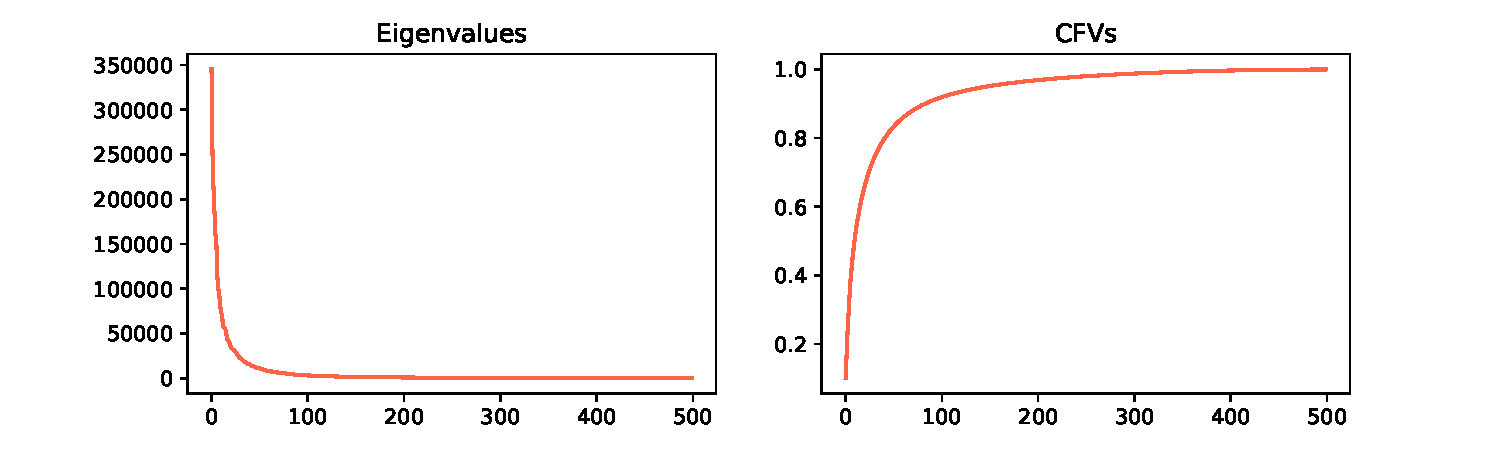
\includegraphics[width=\linewidth]{p2_cfvs}

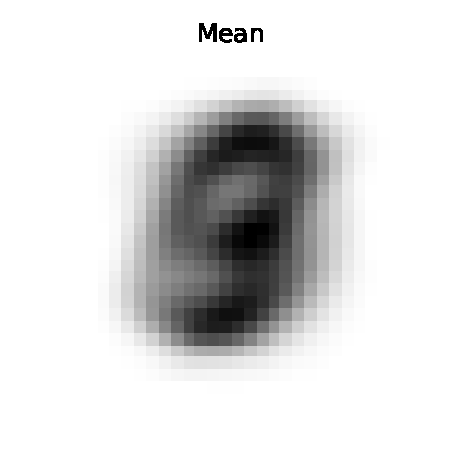
\includegraphics[width=0.25\linewidth]{p2_mean}
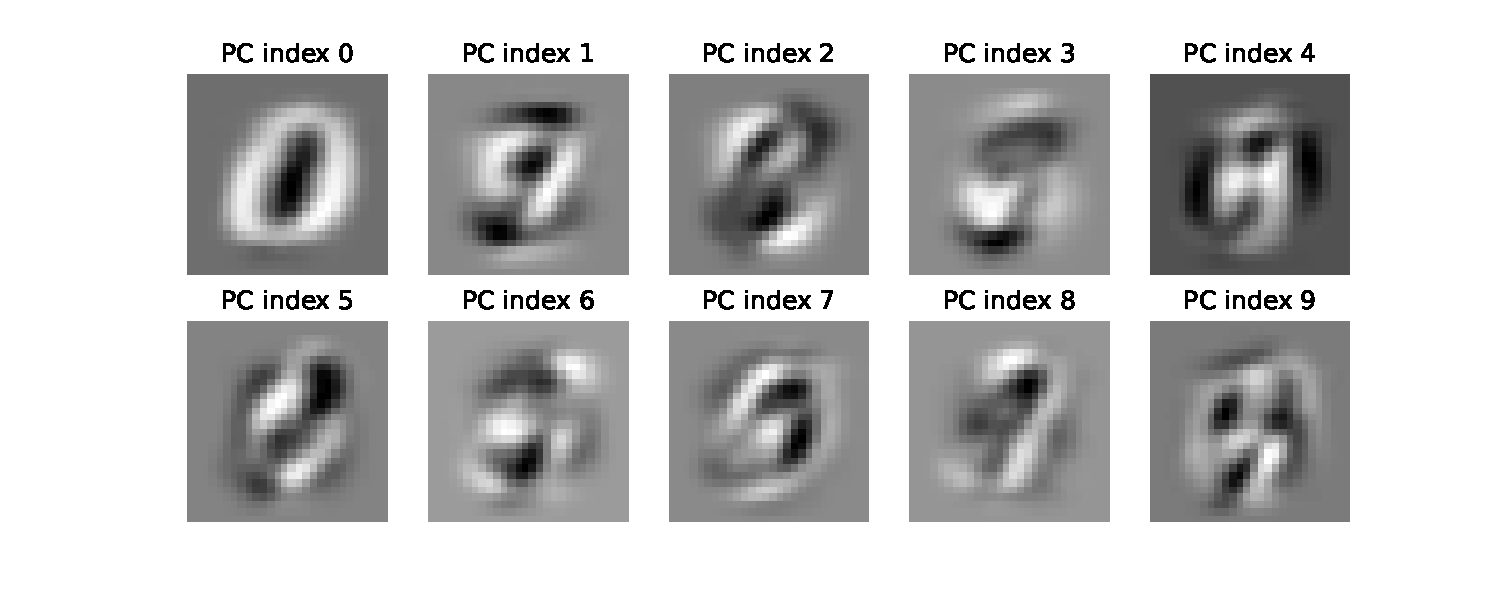
\includegraphics[width=0.75\linewidth]{p2_pcomps}

Code:

\begin{python}
def pca(x, n_comps=500):
    # Center the data by subtracting the mean of each feature
    x = x - x.mean(0)

    # Calculate the empirical covariance matrix
    emp_cov = x.T @ x / x.shape[0]

    # Find the n_comps largest eigenvalues and corresponding eigenvectors
    U, S, Vh = torch.linalg.svd(emp_cov)
    top_eigvals = S[:n_comps]
    top_pcomps = U.T[:n_comps] # eigenvectors are cols of U
    return top_eigvals, top_pcomps


def calc_cfvs(eigvals):
    cum_frac_vars = torch.cumsum(eigvals, 0) / eigvals.sum()
    return cum_frac_vars


def calc_errs(x, pcomps):
    def calc_err(x, U):
        x = x - x.mean(0) # center the data
        z = x @ U.T # embeddings
        err = (torch.linalg.norm(x - z @ U, 1) ** 2).mean(0)
        return err
    err_mean = calc_err(x, torch.zeros((1, x.shape[1]))) # mean - mean = 0
    err_pcomp = calc_err(x, pcomps[:10])
    return err_mean, err_pcomp
\end{python}

\begin{enumerate}
  \item From the second plot, nearly all of the variance is explained by the first 500 components, since the cumulative proportion is nearly at $k=500$ is almost 1. The cumulative proportion of variance increases with $k$, very rapidly until about $k=50$, where it reaches an ``elbow" point in the graph and begins to increase much more slowly, until it finally reaches 1 when $k$ is equal to the original dimension of the data.

  \item The principle component images are similar to the cluster centers from K-means, particularly the cluster centers from K-means with standardized data, in that they vaguely resemble digits from 0-9, but the principle component images are generally blurrier and correspond less clearly to digits than the K-means cluster centers, with the first PC clearly representing ``0", a few of the PCs looking like ``9", and the rest looking like blurry ``8"s or amorphous blobs. This blurriness is partly because only the first ten PCs do not approximate the images well enough and partly because PCA generally results in less interpretable parameters than K-means.

  \item
  \texttt{Reconstruction error (using mean): 4.263164e+11 \\
  	Reconstruction error (using mean and top 10 pcomps): 1.880565e+11}

  For comparison, the final residual sum of squares objective loss I achieved by using K-means on the dataset was less than 1.30e+10.
  
  \TODO come back when HW4 solns are released to check against K-means loss

  \item No, this would not change the quality of reconstruction error in the last problem, provided that the $z_n$ was recalculated accordingly for each data point $x_n$. This is because multiplying $U$ by a rotation matrix $R$ still gives an orthogonal matrix whose components span the subspace spanned by the $k$ eigenvectors in $U$. However, the interpretation of the components would change, because each component no longer corresponds to a direction of greatest variance in the data, since they have been rotated.
\end{enumerate}

\newpage

\begin{problem}[Bayesian Networks, 10 pts]

% FDV: I think we can keep this problem as-is, and just clarfiy based
% on notes from last year.
% # problem 3 clarifications
% The phrasing of Q3 is slightly off because it implies that you need to explain why each path is not blocked in the case that two nodes are not independent. It is sufficient to provide a single unblocked path. Better phrasing is (emphasis added) "Use the concept of d-separation to answer the questions and show your work (i.e., state what the blocking path(s) is/are and which node blocks the path; or explain why there exists a path that is not blocked)." 
% 
% Some helpful resources for d-separation:  The 2020 Section 8 notes, Bishop p. 372 - 379, Section 8.2 of the CS 181 textbook
% 
% Problem 3: Make it clear (put the instructions in one place) that we require explanations for both "yes" and "no" answers

  
  \noindent In this problem we explore the conditional independence
  properties of a Bayesian Network.  Consider the following Bayesian
  network representing a fictitious person's activities. Each random
  variable is binary (true/false).

\begin{center}
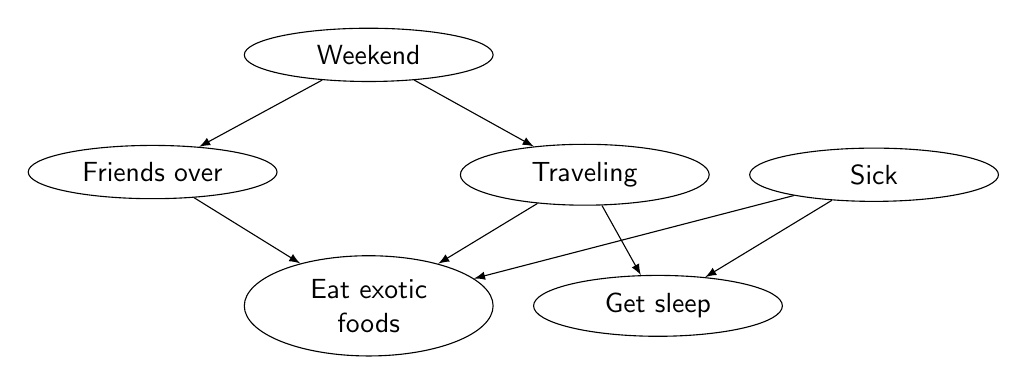
\begin{tikzpicture}[
  node distance=1cm and .5cm,
  bn/.style={draw,ellipse,text width=2cm,align=center}
    ]
    \node[bn] (w) {\attr{Weekend}};
    \node[bn,below right=of w] (t) {\attr{Traveling}};
    \node[bn,right=of t] (s) {\attr{Sick}};
    \node[bn,below left=of w] (f) {\attr{Friends over}};
    \node[bn,below right=of f] (eef) {\attr{Eat exotic foods}};
    \node[bn,right=of eef] (gs) {\attr{Get sleep}};
    \path (w) edge[-latex] (t)
    (w) edge[-latex] (f)
    (f) edge[-latex] (eef)
    (t) edge[-latex] (eef)
    (t) edge[-latex] (gs)
    (s) edge[-latex] (gs)
    (s) edge[-latex] (eef);
    \end{tikzpicture}
\end{center}

The random variables are:

\begin{itemize}
\item \attr{Weekend}: Is it the weekend?
\item \attr{Friends over}: Does the person have friends over?
\item \attr{Traveling}: Is the person traveling?
\item \attr{Sick}: Is the person sick?
\item \attr{Eat exotic foods}: Is the person eating exotic foods?
\item \attr{Get Sleep}: Is the person getting sleep?
\end{itemize}

\medskip

For the following questions, $A \perp B$ means that events A and B are
independent and $A \perp B | C$ means that events A and B are independent
conditioned on C.

\textbf{Use the concept of d-separation} to answer the
questions and show your work (i.e., state what the blocking path(s) is/are and what nodes block the path; or explain why each path is not blocked).

\textit{Example Question:} Is $\attr{Friends over} \perp \attr{Traveling}$? If NO, give intuition for why.

\textit{Example Answer:} NO. The path from Friends over -- Weekend -- Traveling is not blocked following the d-separation rules as we do not observe Weekend. Thus, the two are not independent. 

\textbf{Actual Questions:}

\begin{enumerate}
\item Is $\attr{Weekend} \perp \attr{Get Sleep}$?
  If NO, give intuition for why.

\item Is $\attr{Sick} \perp \attr{Weekend}$?
  If NO, give intuition for why.


\item Is $\attr{Sick} \perp \attr{Friends over}\given \attr{Eat exotic
  foods}$? If NO, give intuition for why.


\item Is $\attr{Friends over} \perp \attr{Get Sleep}$? If NO, give
  intuition for why.

\item Is $\attr{Friends over} \perp \attr{Get Sleep} \given
  \attr{Traveling}$? If NO, give intuition for why.

\item Suppose the person stops traveling in ways that affect their
  sleep patterns.  Travel still
  affects whether they eat exotic foods.  Draw the modified network. (Feel free to reference the handout file for the commands for displaying the new network in \LaTeX).

\item For this modified network, is $\attr{Friends over} \perp
  \attr{Get Sleep}$? If NO, give an intuition why.  If YES,
  describe what observations (if any) would cause them to no longer be
  independent.

\end{enumerate}
\end{problem}

\newpage
\section*{Solution}
\begin{enumerate}
  \item NO. The path $\attr{Weekend} \rightarrow \attr{Traveling} \rightarrow \attr{Get sleep}$ is not blocked because we do not observe $\attr{Traveling}$. For intuition, if it was the weekend, the probability of travel could be increased, which could decrease the probability of getting sleep due to jet lag, etc.
  \item YES. All of the paths between $\attr{Sick}$ and $\attr{Weekend}$ are blocked. The ``sub-path" $\attr{Sick} \rightarrow \attr{Get sleep} \leftarrow \attr{Traveling}$ is blocked because $\attr{Get sleep}$ is not observed, and the ``sub-paths" $\attr{Sick} \rightarrow \attr{Eat exotic foods} \leftarrow \attr{Traveling}$ and $\attr{Sick} \rightarrow \attr{Eat exotic foods} \leftarrow \attr{Friends over}$ are blocked because $\attr{Eat exotic foods}$ is not observed.
  \item NO. The path $\attr{Sick} \rightarrow \attr{Eat exotic foods} \leftarrow \attr{Friends over}$ is unblocked when $\attr{Eat exotic foods}$ is observed.
  For intuition, suppose the person is likely to eat exotic foods when they have friends over or when they are not sick. If we observe that they eat exotic foods, but do not have friends over, then it becomes more likely that they are not sick, due to the ``explaining away" effect.

  \item NO. The path $\attr{Friends over} \leftarrow \attr{Weekend} \rightarrow \attr{Traveling} \rightarrow \attr{Get sleep}$ is not blocked, since $\attr{Friends over} \leftarrow \attr{Weekend} \rightarrow \attr{Traveling}$ is not blocked given that $\attr{Weekend}$ is unobserved and $\attr{Weekend} \rightarrow \attr{Traveling} \rightarrow \attr{Get sleep}$ is not blocked given that $\attr{Traveling}$ is not observed. For intuition, if the person had friends over, it could increase the probability of $\attr{Weekend}$, which could increase the probability of $\attr{Traveling}$, which could in turn decrease the probability of $\attr{Get sleep}$.
  
  \item YES. The path $\attr{Friends over} \leftarrow \attr{Weekend} \rightarrow \attr{Traveling} \rightarrow \attr{Get sleep}$ is blocked, since $\attr{Weekend} \rightarrow \attr{Traveling} \rightarrow \attr{Get sleep}$ is blocked given that $\attr{Traveling}$ is observed. The other possible paths, $\attr{Friends over} \rightarrow \attr{Eat exotic foods} \leftarrow \attr{Traveling} \rightarrow \attr{Get sleep}$ and $\attr{Friends over} \rightarrow \attr{Eat exotic foods} \leftarrow \attr{Sick} \rightarrow \attr{Get sleep}$, are blocked because $\attr{Friends over} \rightarrow \attr{Eat exotic foods} \leftarrow \attr{Traveling}$ and $\attr{Friends over} \rightarrow \attr{Eat exotic foods} \leftarrow \attr{Sick}$ are blocked given that $\attr{Eat exotic foods}$ is not observed.
  
  \item Removing the edge from $\attr{Traveling}$ to $\attr{Get sleep}$, the modified network is as follows.

  \begin{center}
  	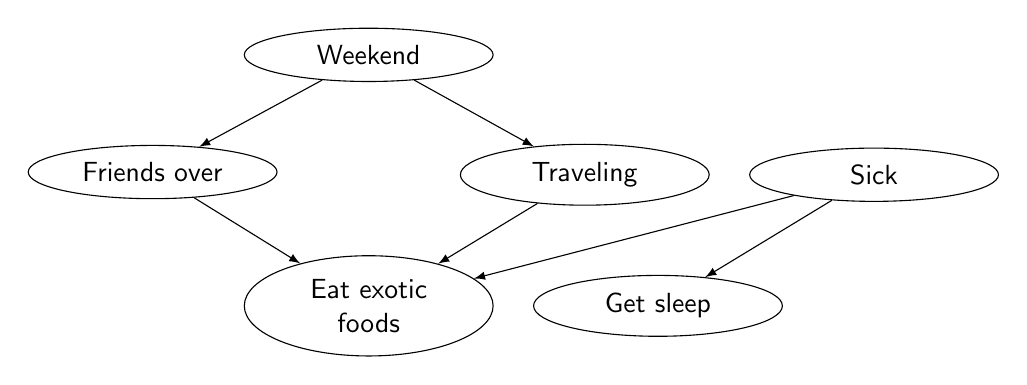
\begin{tikzpicture}[
  		node distance=1cm and .5cm,
  		bn/.style={draw,ellipse,text width=2cm,align=center}
  		]
  		\node[bn] (w) {\attr{Weekend}};
  		\node[bn,below right=of w] (t) {\attr{Traveling}};
  		\node[bn,right=of t] (s) {\attr{Sick}};
  		\node[bn,below left=of w] (f) {\attr{Friends over}};
  		\node[bn,below right=of f] (eef) {\attr{Eat exotic foods}};
  		\node[bn,right=of eef] (gs) {\attr{Get sleep}};
  		\path (w) edge[-latex] (t)
  		(w) edge[-latex] (f)
  		(f) edge[-latex] (eef)
  		(t) edge[-latex] (eef)
  		(s) edge[-latex] (gs)
  		(s) edge[-latex] (eef);
  	\end{tikzpicture}
  \end{center}

  \item YES. The only path is $\attr{Friends over} \rightarrow \attr{Eat exotic foods} \leftarrow \attr{Sick} \rightarrow \attr{Get sleep}$, which is blocked because $\attr{Friends over} \rightarrow \attr{Eat exotic foods} \leftarrow \attr{Sick}$ is blocked given that $\attr{Eat exotic foods}$ is not observed. Observing $\attr{Eat exotic foods}$ would unblock this path, causing $\attr{Friends over}$ and $\attr{Get sleep}$ to no longer be independent, since $\attr{Eat exotic foods} \leftarrow \attr{Sick} \rightarrow \attr{Get sleep}$ is already unblocked given that $\attr{Sick}$ is not observed.
\end{enumerate}

\newpage
%%%%%%%%%%%%%%%%%%%%%%%%%%%%%%%%%%%%%%%%%%%%%
% Name and Calibration
%%%%%%%%%%%%%%%%%%%%%%%%%%%%%%%%%%%%%%%%%%%%%
\subsection*{Name}

Alex Encalada-Stuart

\subsection*{Collaborators and Resources}
Whom did you work with, and did you use any resources beyond cs181-textbook and your notes?

No one and none

\subsection*{Calibration}
Approximately how long did this homework take you to complete (in hours)? 

20

\end{document}
